\documentclass[aps,prper,amsmath,amssymb,nofootinbib,12pt]{revtex4-2}
\usepackage{amsmath,amssymb,amsfonts}
\usepackage{tikz}
\usetikzlibrary{calc, arrows.meta, positioning}
\usepackage{xcolor}

\begin{document}

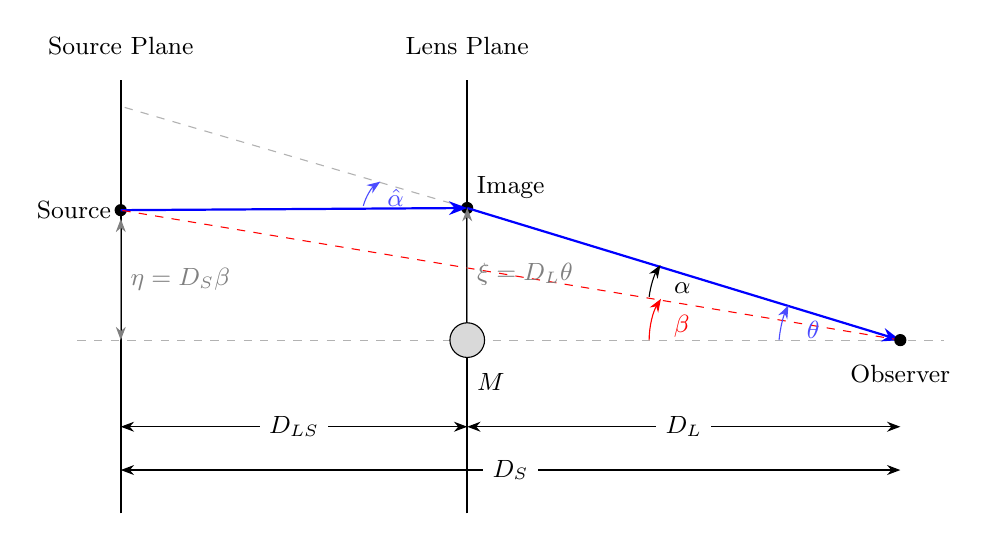
\begin{tikzpicture}[
	scale=1.1,
	>=Stealth,
	every node/.style={font=\small},
	plane/.style={thick, black},
	optical axis/.style={dashed, gray!60},
	light ray/.style={blue, thick, ->},
	undeflected/.style={red, dashed, thin},
	extension/.style={gray, dashed, very thin},
	angle arc/.style={->, >=Stealth, blue!70}
	]
	% =====================================================
	% KOORDINAT UTAMA (Konvensi standar: Observer di kanan)
	% =====================================================
	\coordinate (Observer) at (0,0);
	\coordinate (LensPlane) at (-5,0);
	\coordinate (SourcePlane) at (-9,0);
	\coordinate (Source) at (-9,1.5);
	\coordinate (Image) at (-5,1.525);
	\coordinate (Image_2) at (-9,2.7);

	% =====================================================
	% LABEL JARAK (Angular Diameter Distances)
	% =====================================================
	\draw[<->, black] (0,-1.0) -- (-5,-1.0) node[midway, fill=white] {$D_L$};
	\draw[<->, black] (-5,-1.0) -- (-9,-1.0) node[midway, fill=white] {$D_{LS}$};
	\draw[<->, black] (0,-1.5) -- (-9,-1.5) node[midway, fill=white] {$D_S$};

	\draw[optical axis] (Image) -- (Image_2);


	% =====================================================
	% =====================================================
	\draw[optical axis] (-9.5,0) -- (0.5,0);
	\draw[plane] (-5,-2) -- (-5,3) node[above, yshift=2mm] {Lens Plane};
	\draw[plane] (-9,-2) -- (-9,3) node[above, yshift=2mm] {Source Plane};

	% =====================================================
	% =====================================================
	\fill[black] (Source) circle (2pt) node[left] {Source};
	\fill[black] (Image) circle (2pt) node[above right] {Image};

	% =====================================================
	% JALUR CAHAYA
	% =====================================================
	\draw[light ray] (Source) -- (Image);
	\draw[light ray] (Image) -- (Observer);
	\draw[undeflected] (Observer) -- (Source);

	% =====================================================
	% SUDUT DI POSISI OBSERVER
	% =====================================================
	\draw[angle arc] (-1.4,0) arc (175:155:1.2) node[midway, left, xshift=6mm, yshift=-1mm] {$\theta$};
	\draw[angle arc, red] (-2.9,0) arc (180:148:0.9) node[midway, left, xshift=6mm, yshift=-1mm] {$\beta$};
	\draw[angle arc, black] (-2.9,0.5) arc (173:148:0.9) node[midway, left, xshift=6mm, yshift=-1mm] {$\alpha$};

	% =====================================================
	% SUDUT DEFLEKSI DI LENS PLANE
	% =====================================================
	\draw[angle arc] (-6.2,1.55) arc (165:125:0.5) node[midway, above right, xshift=1mm, yshift=-3mm] {$\hat{\alpha}$};

	% =====================================================
	% JARAK TRANSVERSAL
	% =====================================================
	\draw[<->, gray] (-5,0) -- (-5,1.525) node[midway, right] {$\xi = D_L\theta$};
	\draw[<->, gray] (-9,0) -- (-9,1.4) node[midway, right] {$\eta = D_S\beta$};

	% =====================================================
	% =====================================================
	\fill[black] (Observer) circle (2pt) node[below, yshift=-2mm] {Observer};
	\draw[fill=gray!30] (-5,0) circle (0.2) node[below, xshift=3mm,yshift=-3mm] {$M$};

\end{tikzpicture}

\end{document}